\section{Results and Discussion}
\label{sec:results}

\begin{figure}
	\begin{center}
		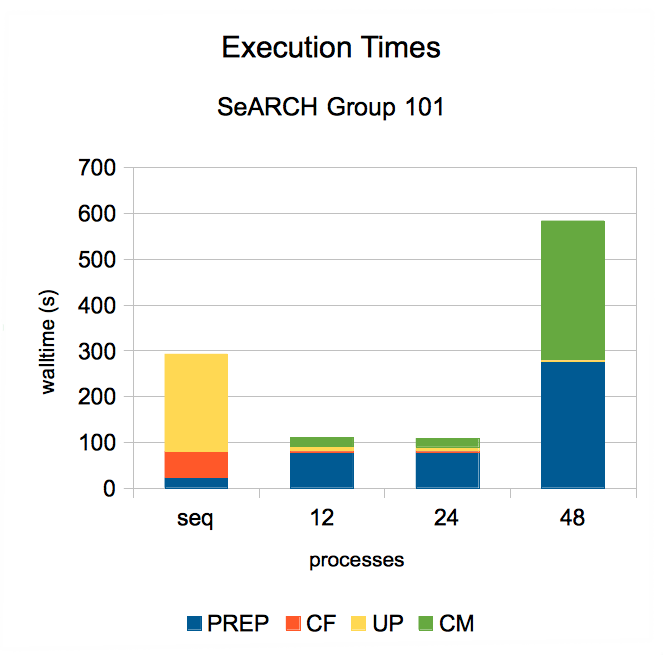
\includegraphics[width=\columnwidth]{report.may/images/exectime101.png}
		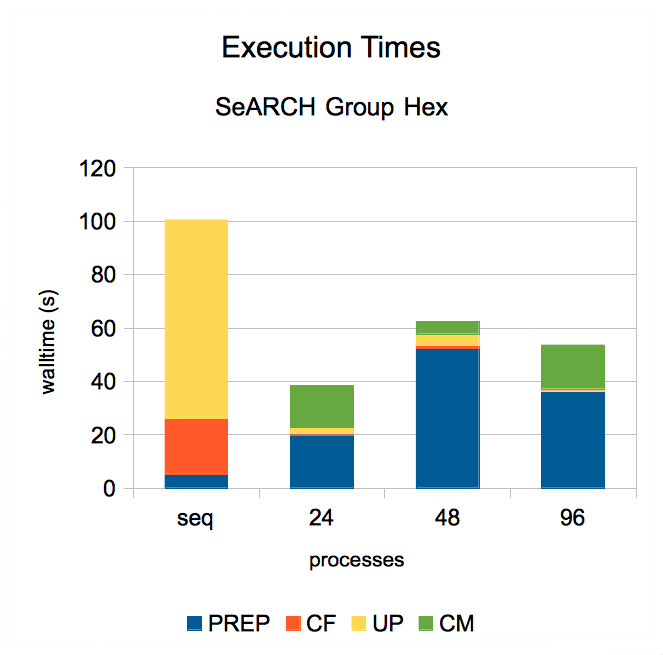
\includegraphics[width=\columnwidth]{report.may/images/exectimehex.png}
		\caption[Execution times]{Execution times of the tests performed on SeARCH Groups 101 and Hex.}
	\end{center}
	\label{fig:exectime}
\end{figure}

\begin{figure}
	\begin{center}
		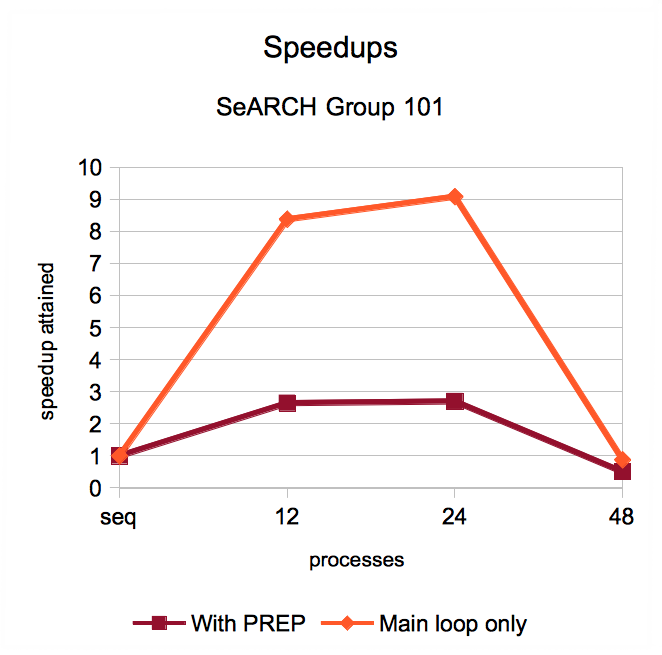
\includegraphics[width=\columnwidth]{report.may/images/speedup101.png}
		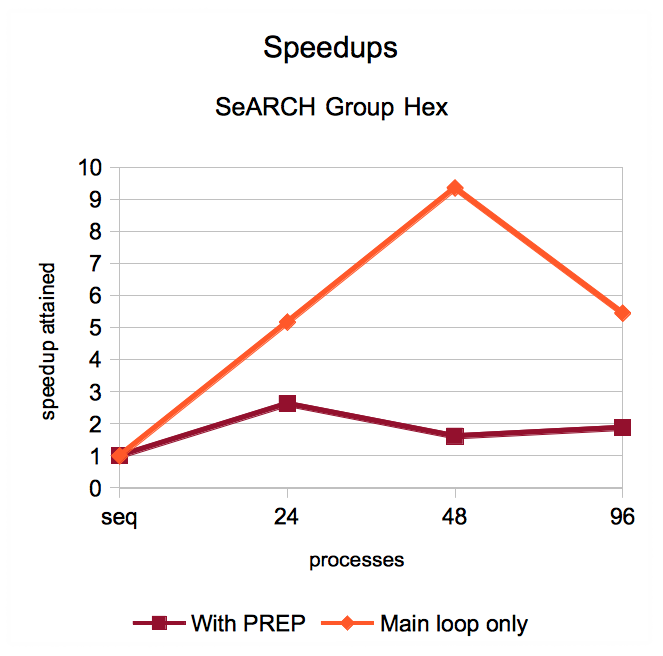
\includegraphics[width=\columnwidth]{report.may/images/speeduphex.png}
		\caption[Speedups]{Speedups achieved for different numbers of processes on SeARCH Groups 101 and Hex.}
	\end{center}
	\label{fig:speedup}
\end{figure}

\begin{figure*}[!t]
	\begin{center}
		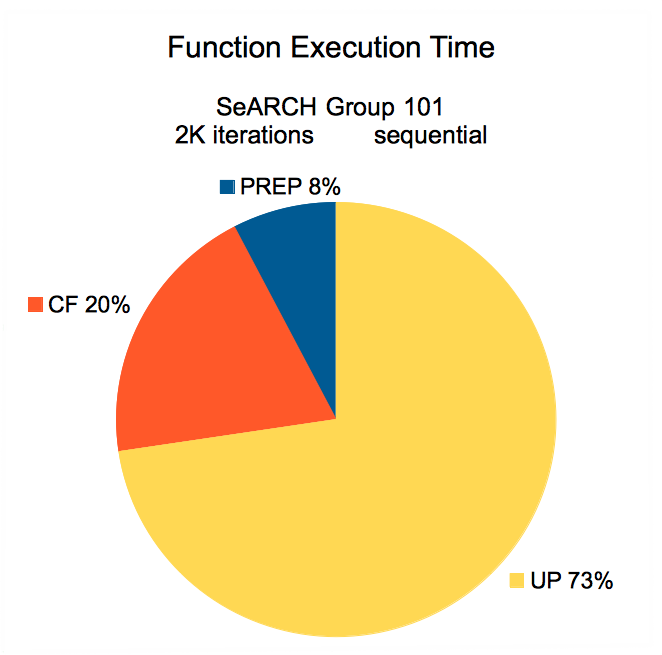
\includegraphics[width=\columnwidth]{report.may/images/loadseq101.png}
		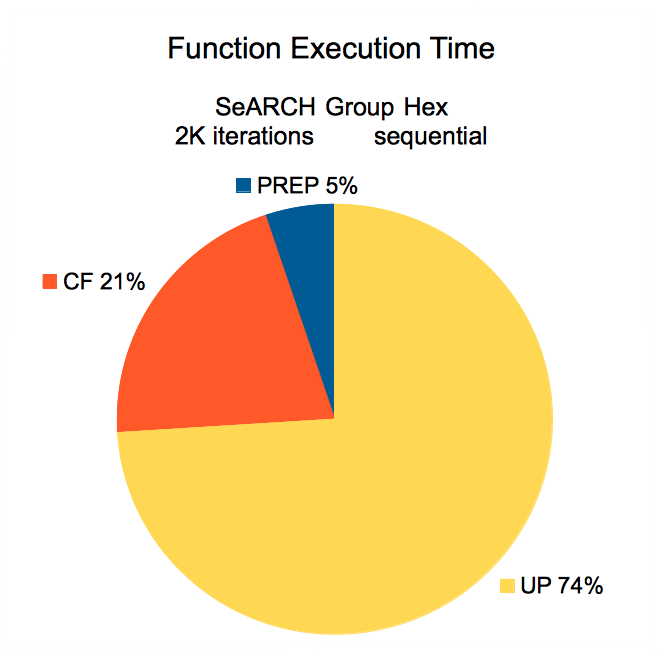
\includegraphics[width=\columnwidth]{report.may/images/loadseqhex.png}
		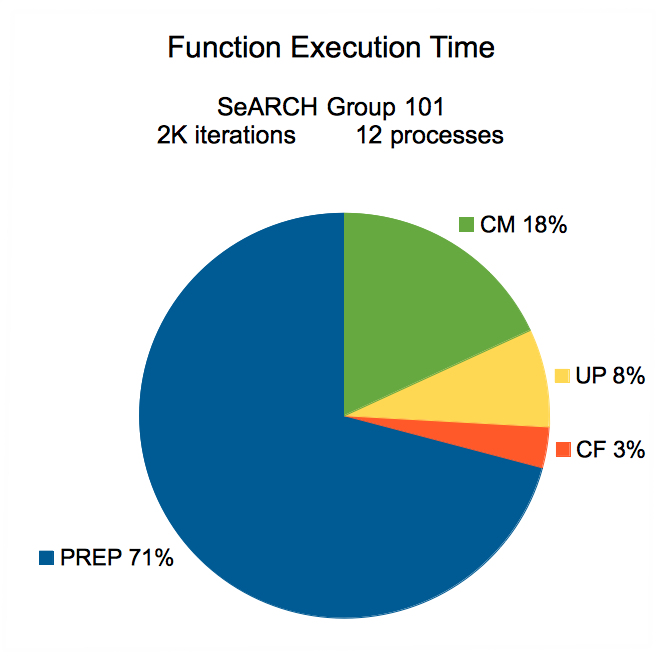
\includegraphics[width=\columnwidth]{report.may/images/load12101.png}
		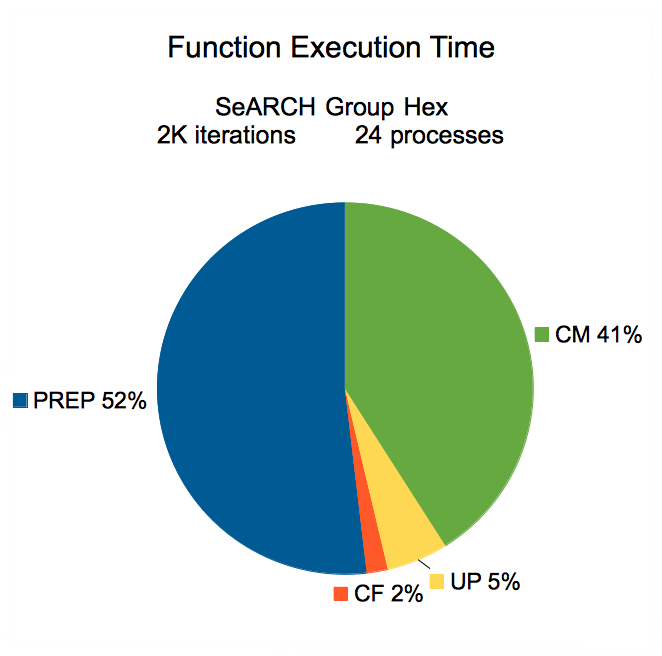
\includegraphics[width=\columnwidth]{report.may/images/load24hex.png}
		\caption[Work loads]{Median work load of each part of the program in an execution, for the sequential version and the MPI version using half of the available hardware threads on SeARCH Groups 101 and Hex.}
	\end{center}
	\label{fig:load1}
\end{figure*}

\begin{figure*}[!t]
	\begin{center}
		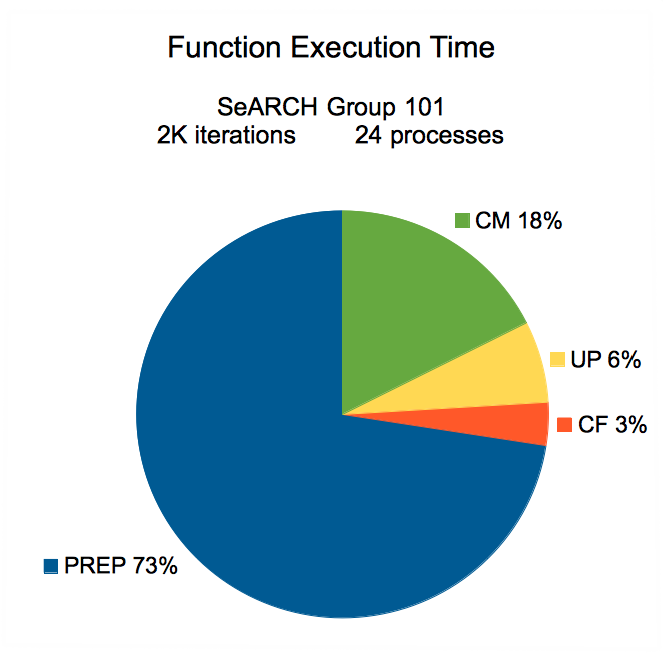
\includegraphics[width=\columnwidth]{report.may/images/load24101.png}
		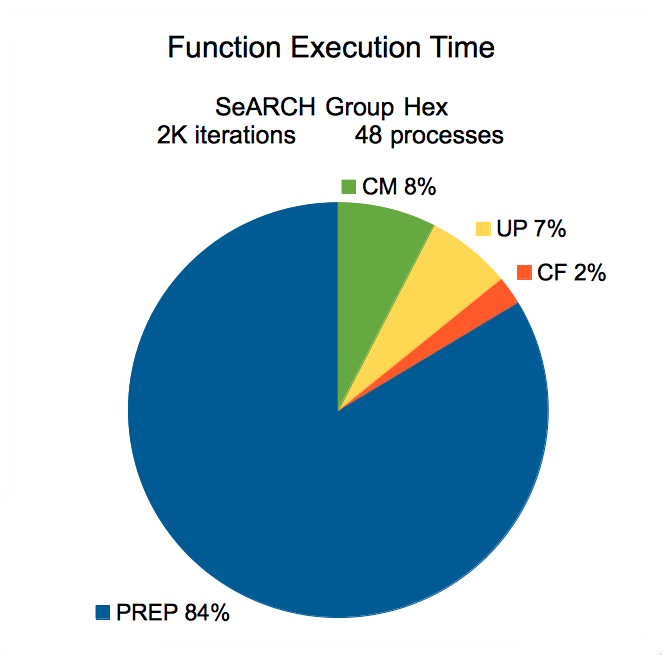
\includegraphics[width=\columnwidth]{report.may/images/load48hex.png}
		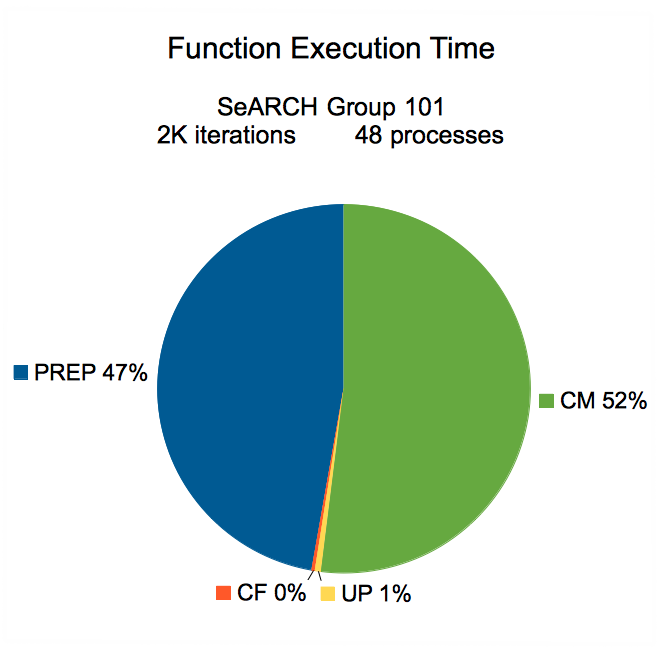
\includegraphics[width=\columnwidth]{report.may/images/load48101.png}
		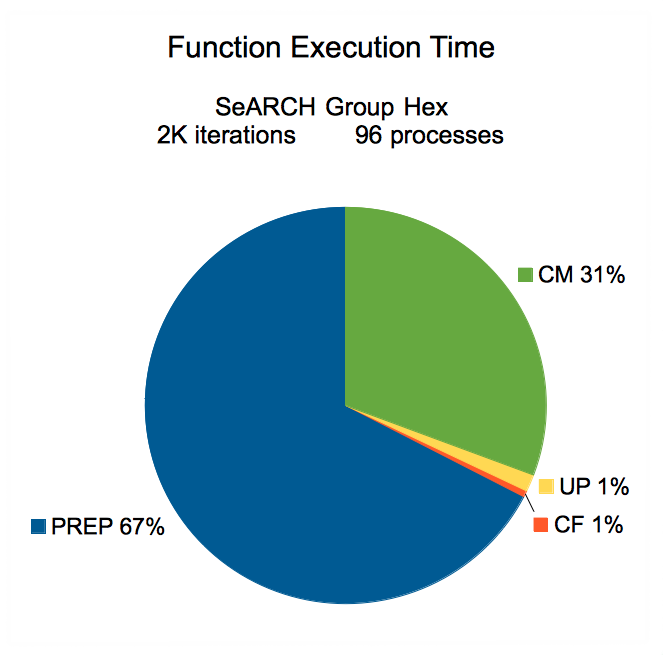
\includegraphics[width=\columnwidth]{report.may/images/load96hex.png}
		\caption[Work loads]{Median work load of each part of the program in an execution, for the MPI version issuing processes in the exact number and the double of the available hardware threads on SeARCH Groups 101 and Hex.}
	\end{center}
	\label{fig:load2}
\end{figure*}